\subsection{Panoramica UCS4}

\begin{figure}[h]
	\centering	
	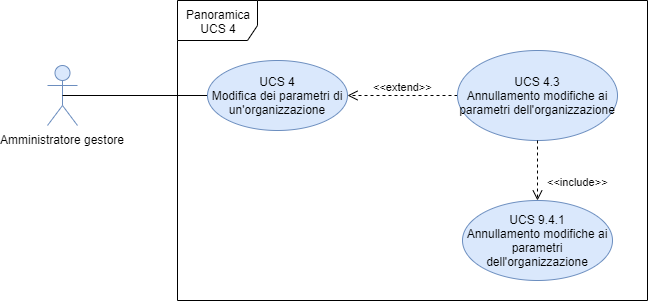
\includegraphics[scale=0.53]{sezioni/UseCase/Immagini/PS4.png}
	\caption{Panoramica UCS 4}
\end{figure}

\subsubsection{UCS 4 - Modifica dei parametri dell'organizzazione}%kite level

\begin{figure}[h]
	\centering	
	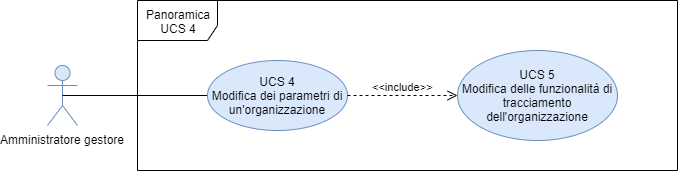
\includegraphics[scale=0.53]{sezioni/UseCase/Immagini/UCS4.png}
	\caption{UCS 4 - Modifica dei parametri dell'organizzazione}
\end{figure}

\begin{itemize}
    \item \textbf{Attori primari:} Amministratore gestore
    \item \textbf{Precondizione:} L’amministratore dispone di almeno un'organizzazione.
    \item \textbf{Postcondizione:} L’amministratore ha modificato i parametri desiderati dell'organizzazione e le modifiche sono state salvate nel sistema.
    \item \textbf{Scenario principale:} L'amministratore deve scegliere l'organizzazione che vuole modificare, selezionare la funzionalità di modifica dell'organizzazione e quindi procedere con il cambiamento dei parametri.
    \item \textbf{Scenario alternativo:} L'amministratore non vuole più apportare modifiche all'organizzazione, pertanto procederà con l'annullamento dell'apporto di modifiche [UCS 4.3].
    \item \textbf{Flusso di eventi:}
    \begin{enumerate}
        \item L'amministratore seleziona un'organizzazione [UCS 3];
        \item L'amministratore seleziona la funzionalità di modifica dell'organizzazione;
        \item L'amministratore ha la possibilità di modificare i campi delle informazioni dell’organizzazione [UCS 4.1];
        \item L'amministratore ha la possibilità di modificare il perimetro\ap{G} e i luoghi\ap{G} di tracciamento dell’organizzazione [UCS 5];
        \item L'amministratore seleziona la funzionalità per il salvataggio delle modifiche apportate.
    \end{enumerate}
    \item \textbf{Estensioni:}
    \begin{enumerate}
        \item UCS 4.3 - Annullamento modifiche ai parametri dell'organizzazione.
    \end{enumerate}
\end{itemize}

\subsubsection{UCS 4.1 - Modifica dei dati dell'organizzazione}%sea level
\begin{figure}[h]
	\centering
    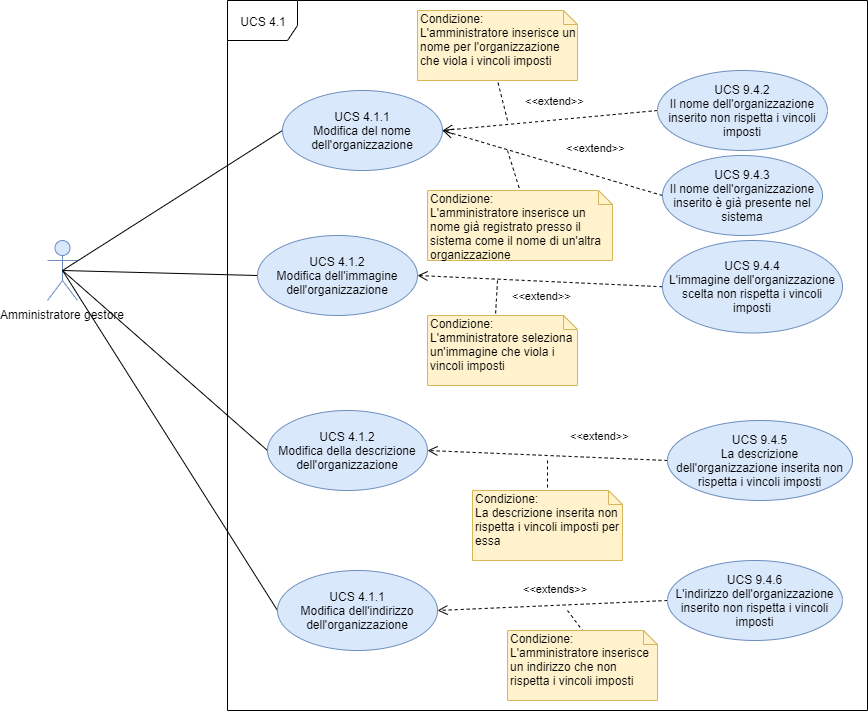
\includegraphics[scale=0.53]{sezioni/UseCase/Immagini/UCS4.1.png}
    \caption{UCS 4.1 - Modifica dei dati dell'organizzazione}
\end{figure}
\begin{itemize}
    \item \textbf{Attori primari:} Amministratore gestore
    \item \textbf{Precondizione:} L'amministratore si trova nella sezione di modifica dei parametri dell'organizzazione.
    \item \textbf{Postcondizione:} L'amministratore ha modificato i dati desiderati all'interno dell’organizzazione.
    \item \textbf{Scenario principale:} L'amministratore modifica i dati dell'organizzazione desiderati, ovvero può:
    \begin{itemize}
        \item modificare il nome dell'organizzazione [UCS 4.1.1];
        \item modificare l'immagine dell'organizzazione [UCS 4.1.2];
        \item modificare la descrizione dell'organizzazione [UCS 4.1.3];
        \item modificare l'indirizzo dell'organizzazione [UCS 4.1.4].
    \end{itemize}
\end{itemize}

\subsubsection{UCS 4.1.1 - Modifica del nome dell'organizzazione}%fish level
\begin{itemize}
\item \textbf{Attori primari:} Amministratore gestore
\item \textbf{Precondizione:} L'amministratore gestore si trova nella sezione di modifica dei parametri dell'organizzazione.
\item \textbf{Postcondizione:} L'amministratore ha inserito un nome per l'organizzazione che rispetti i vincoli imposti e non sia già presente nel sistema.
\item \textbf{Scenario alternativo 1:} L'amministratore inserisce un nome per l'organizzazione che non rispetta i vincoli imposti. Verrà visualizzato un messaggio d'errore [UCS 9.4.2].
\item \textbf{Scenario alternativo 2:} L'amministratore inserisce un nome per l'organizzazione che è gia presente nel sistema. Verrà visualizzato un messaggio d'errore [UCS 9.4.3].
\item \textbf{Estensioni:}
\begin{enumerate}
    \item UCS 9.4.2 - Il nome dell'organizzazione inserito non rispetta i vincoli;
    \item UCS 9.4.3 - Il nome dell'organizzazione inserito è già presente nel sistema.
\end{enumerate}
\end{itemize}

\subsubsection{UCS 4.1.2 - Modifica dell'immagine dell'organizzazione}%fish level
\begin{itemize}
\item \textbf{Attori primari:} Amministratore gestore
\item \textbf{Precondizione:} L'amministratore gestore si trova nella sezione di modifica dei parametri dell'organizzazione.
\item \textbf{Postcondizione:} L'amministratore ha selezionato un'immagine valida per l'organizzazione.
\item \textbf{Scenario alternativo:} L'amministratore seleziona un'immagine per l'organizzazione che non rispetta i vincoli imposti. Verrà visualizzato un messaggio d'errore [UCS 9.4.4].
\item \textbf{Flusso di eventi:}
\begin{enumerate}
    \item L'amministratore seleziona la funzionalità di scelta dell'immagine;
    \item Seleziona l'immagine da impostare come immagine dell'organizzazione;
    \item Conferma la scleta.
\end{enumerate}
\item \textbf{Estensioni:}
\begin{enumerate}
    \item UCS 9.4.4 - L'immagine dell'organizzazione scelta non rispetta i vincoli imposti.
\end{enumerate}
\end{itemize}

\subsubsection{UCS 4.1.3 - Modifica della descrizione dell'organizzazione}%fish level
\begin{itemize}
\item \textbf{Attori primari:} Amministratore gestore
\item \textbf{Precondizione:} L'amministratore gestore si trova nella sezione di modifica dei parametri dell'organizzazione.
\item \textbf{Postcondizione:} L'amministratore ha inserito una descrizione che rispetti i vincoli imposti.
\item \textbf{Scenario alternativo:} L'amministratore inserisce una descrizzione dell'organizzazione che non rispetta i vincoli imposti. Verrà visualizzato un messaggio d'errore [UCS 9.4.5].
\item \textbf{Estensioni:}
\begin{enumerate}
    \item UCS 9.4.5 - La descrizione dell'organizzazione inserita non rispetta i vincoli.
\end{enumerate}
\end{itemize}

\subsubsection{UCS 4.1.4 - Modifica dell'indirizzo dell'organizzazione}%fish level

\begin{itemize}
\item \textbf{Attori primari:} Amministratore gestore
\item \textbf{Precondizione:} L'amministratore gestore si trova nella sezione di modifica dei parametri dell'organizzazione.
\item \textbf{Postcondizione:} L'amministratore ha inserito un indirizzo valido che rispetti i vincoli imposti.
\item \textbf{Scenario alternativo:} L'amministratore inserisce un indirizzo dell'organizzazione che non rispetta i vincoli imposti. Verrà visualizzato un messaggio d'errore [UCS 9.4.6].
\item \textbf{Flusso di eventi:}
\begin{enumerate}
    \item L'amministratore inserisce una parola tra: via/viale/piazza;
    \item L'amministratore inserisce il nome della via/viale/piazza dell'azienda;
    \item L'amministratore inserisce il numero civico;
    \item Se serve, l'amministratore inserisce la lettera che identifica l'azienda dagli altri edifici che condividono lo stesso numero civico con essa.
\end{enumerate}
\item \textbf{Estensioni:}
\begin{enumerate}
    \item UCS 9.4.6 - L'indirizzo inserito non rispetta i vincoli imposti.
\end{enumerate}
\end{itemize}

\subsubsection{UCS 4.2 - Richiesta di eliminazione di un'organizzazione}%sea level
\begin{itemize}
\item \textbf{Attori primari:} Amministratore owner
\item \textbf{Precondizione:} L'amministratore si trova nella sezione di modifica dei parametri dell'organizzazione.
\item \textbf{Postcondizione:} L'amministratore ha inviato con successo la richiesta di eliminazione dell'organizzazione.
\item \textbf{Scenario principale:} L'amministratore spiegherà il motivo per cui vuole eliminare l'organizzazione e quindi confermerà l'invio della richiesta.
\item \textbf{Flusso di eventi:}
\begin{enumerate}
    \item L'amministratore seleziona la funzionalità di richiesta di eliminazione dell'organizzazione;
    \item L'amministratore inserisce la motivazione che lo ha spinto a richiedere l'eliminazione dell'organizzazione [UCS 4.2.1];
    \item L'amministratore seleziona la funzionalità di conferma dell'invio della richiesta di eliminazione dell'organizzazione.
\end{enumerate}
\begin{itemize}
    \item UCS 4.2.1 - Motivazione della richiesta dell'eliminazione di un'organizzazione.
\end{itemize}
\end{itemize}

\subsubsection{UCS 4.2.1 - Motivazione della richiesta dell'eliminazione di un'organizzazione}%sea level
\begin{itemize}
\item \textbf{Attori primari:} Amministratore owner
\item \textbf{Precondizione:} L'amministratore si trova nella sezione di modifica dei parametri dell'organizzazione.
\item \textbf{Postcondizione:} L'amministratore ha inserito la motivazione della richiesta di eliminazione dell'organizzazione.
\item \textbf{Scenario principale:} L'amministratore spiegherà il motivo per cui vuole eliminare l'organizzazione.
\end{itemize}

\subsubsection{UCS 4.3 - Annullamento modifiche ai parametri dell'organizzazione}%sea level
\begin{itemize}
\item \textbf{Attori primari:} Amministratore gestore
\item \textbf{Precondizione:} L'amministratore gestore si trova nella sezione di modifica dei parametri dell'organizzazione.
\item \textbf{Postcondizione:} L'amministratore ha annullato le modifiche ai parametri dell'organizzazione.
\item \textbf{Scenario principale:} L'amministratore procederà ad annullare le modifiche ai parametri dell'organizzazione che sta apportando.
\item \textbf{Flusso di eventi:}
\begin{enumerate}
    \item L'amministratore seleziona la funzionalità per annullare le modifiche e tornare alla sezione di gestione dell'organizzazione.
\end{enumerate}
\item \textbf{Inclusioni:}
\begin{enumerate}
    \item UCS 9.4.1 - Visualizzazione del messaggio di conferma di annullamento modifiche.
\end{enumerate}
\end{itemize}